\chapter{Direct Digital Synthesis Jiter} \label{App:DDSJitter}
The DDS IP was tested in order to see how different settings affect output jitter. The only difference in these tests is the length of the frequency control word. The input clock signal is a \SIQ{50}{\mega\hertz} clock signal.

The system is expected to take 10000 samples and with a sample frequency of \SIQ{1}{\mega\hertz} this means the last sample will be taken \SIQ{10}{\milli\second} after the initial acquisition. All the measurements are taken with a \SIQ{20}{\milli\second} delay in order to see an absolute worst case in the sample jitter, note how this is twice the expected sample size. The output of the DDS module for a 32 bit frequency control word can be seen on figure \refq{fig:A_DDS_JITTER_32BIT}.

\begin{figure}[H]
    \centering
    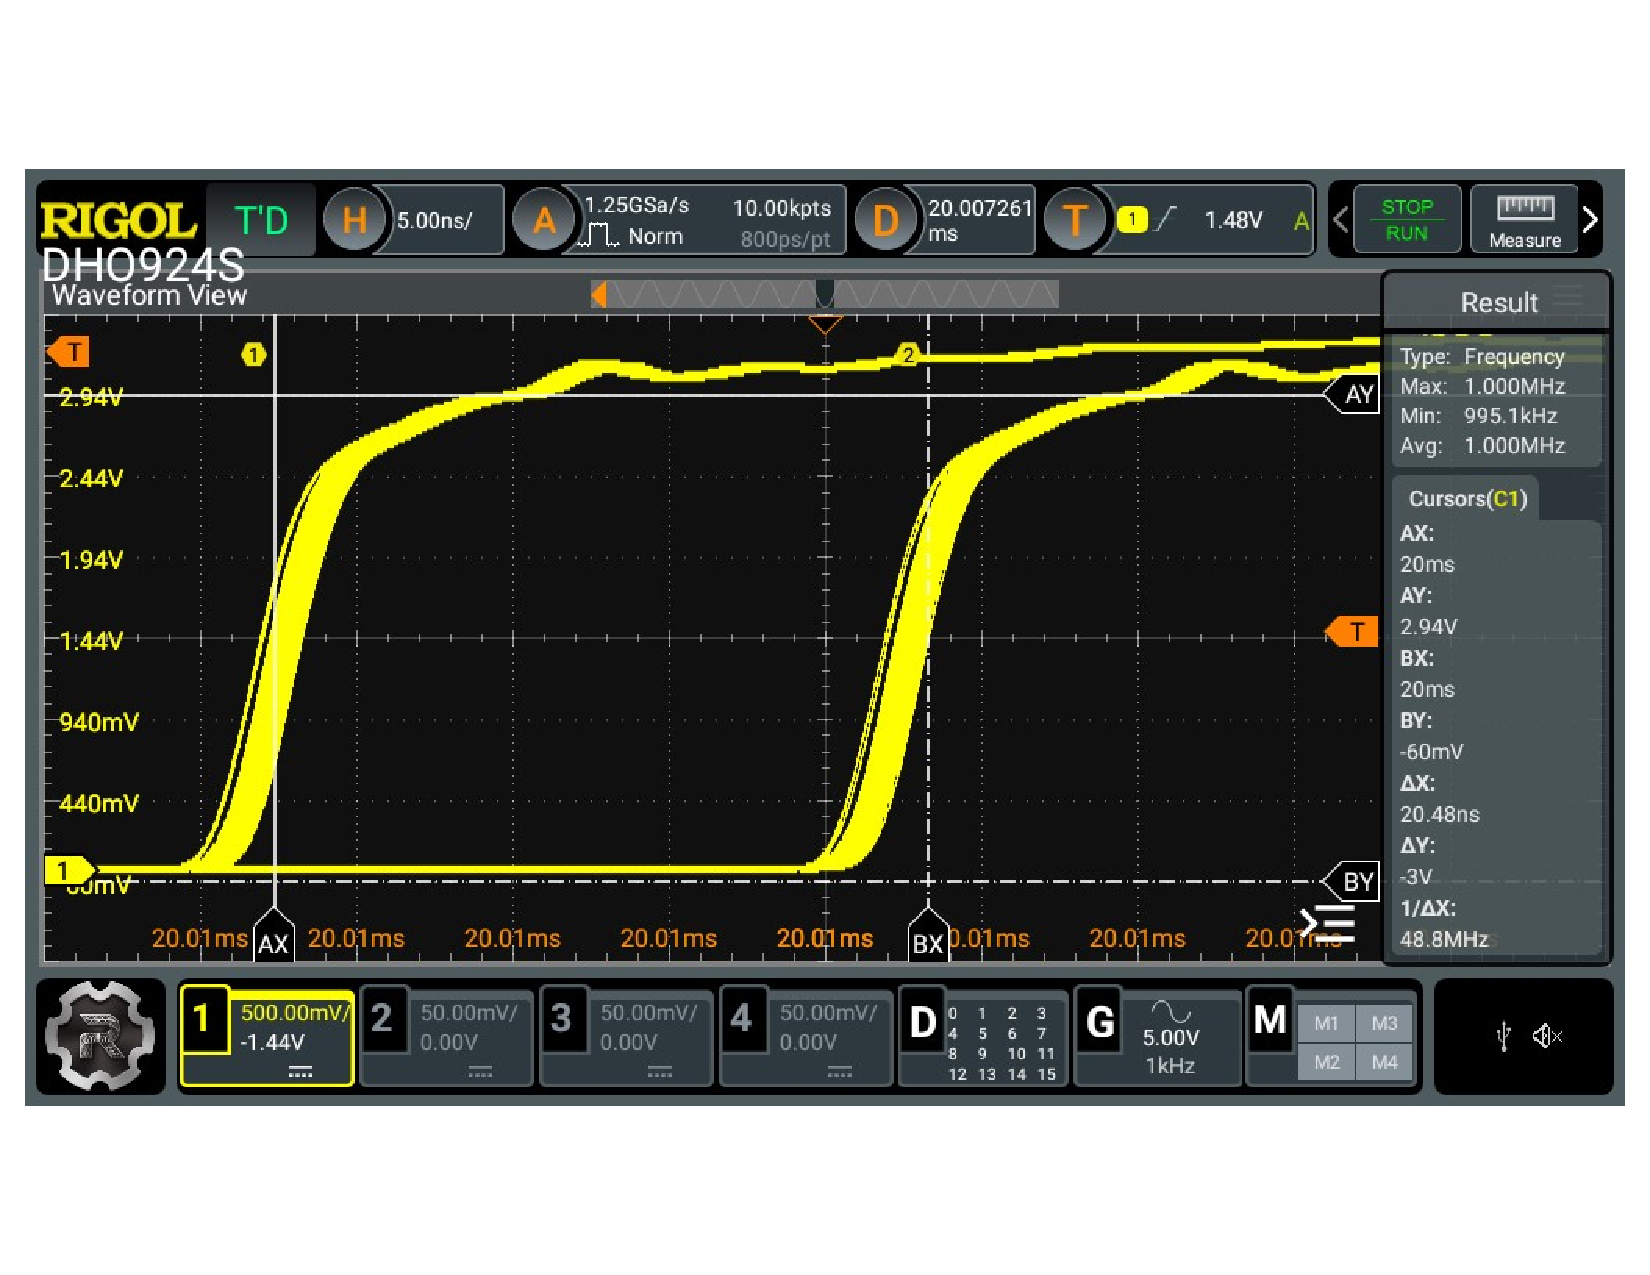
\includegraphics[clip, trim=0 50 0 0, width=0.9\textwidth]{Appendix/Figures/A_DDS_JITTER_32BIT.pdf}
    \caption{A measurement of the output jitter from the DDS block using a 32 bit frequency control word. There is \SIQ{20.48}{\nano\second} of output jitter as can be seen in the measurements in the right side of the screen.}
    \label{fig:A_DDS_JITTER_32BIT}
\end{figure}

The output of the DDS module for a 48 bit frequency control word can be seen on figure \refq{fig:A_DDS_JITTER_48BIT}.
\begin{figure}[H]
    \centering
    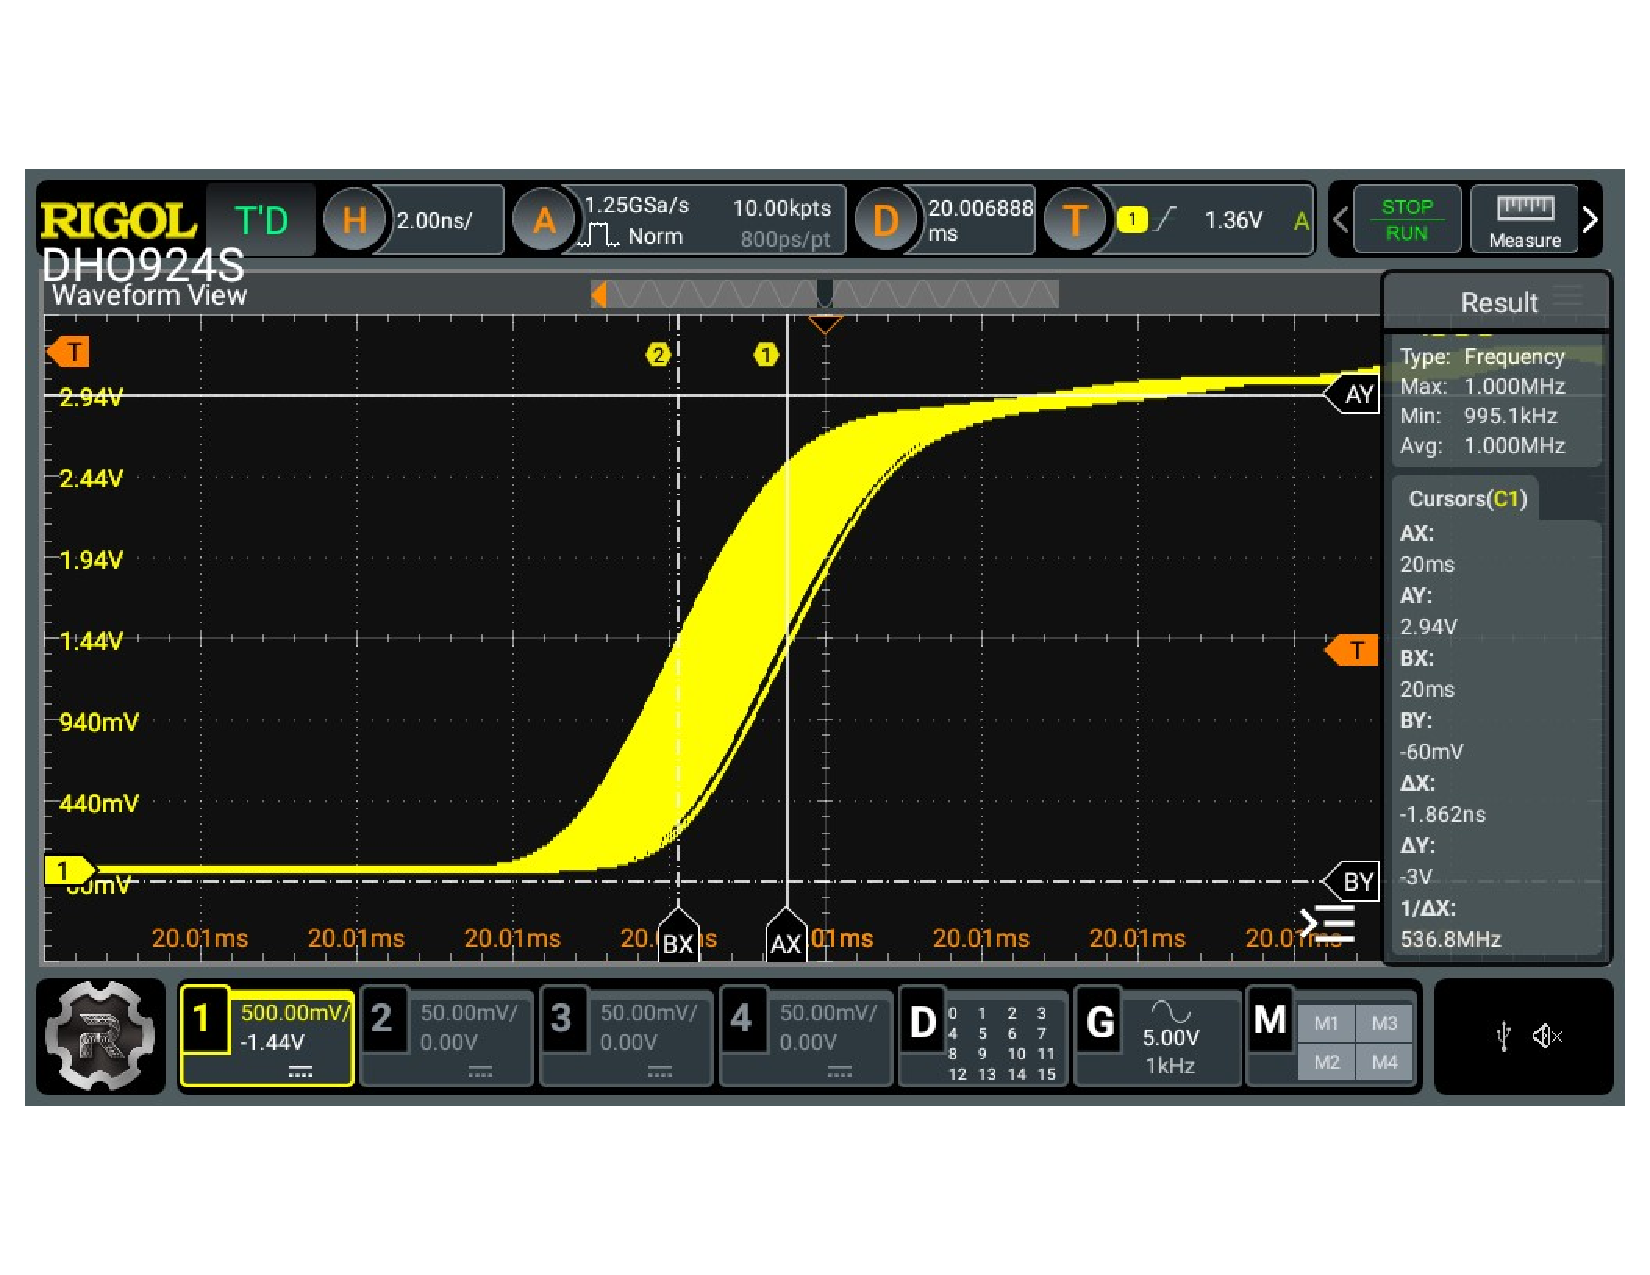
\includegraphics[clip, trim=0 50 0 0, width=0.9\textwidth]{Appendix/Figures/A_DDS_JITTER_48BIT.pdf}
    \caption{A measurement of the output jitter from the DDS block using a 48 bit frequency control word. There is \SIQ{1.862}{\nano\second} of output jitter as can be seen in the measurements in the right side of the screen.}
    \label{fig:A_DDS_JITTER_48BIT}
\end{figure}

Clearly, a larger control word gives better output jitter performance. Note how the output is allowed to "settle" for about 30 seconds before the oscilloscope snapshot was taken. It was noted that the jitter of the 48 bit control word will also grow in size if it is allowed to run for an extended period of time, but a larger control word offers higher performance in the short term in all cases and is thus better for the sampling system.